\chapter{Ermittlungen gegen NS-Verbrechen}

Das Blatt hatte sich längst gewendet -- die einstigen Angreifer, Befehlshaber und Sklavenhalter wurden zu Angeklagten, Gejagten oder Begründern des deutschen Wirtschaftswunders. Letzt\-er\-er Vergleichspunkt scheint abwegig, doch ist er für das Beispiel der Görlitzer WUMAG leider zutreffend.
Während der letzten Kriegswochen sollte die Stadt Görlitz emporsteigen und sich als Festungsinsel der aus Osten kommenden Flut der Rotarmisten behaupten. Durch den Angriff der Roten Armee auf Berlin\index{o}{Berlin} blieb der Stadt Görlitz etwas Zeit, ein klägliches Bollwerk gegen sowjetische Panzer zu errichten und alle Neißebrücken zu sprengen. Die buchstäbliche Drecksarbeit beim Bau der Barrikaden verrichteten die eben aus Rennersdorf zurück beraumten KZ-Häftlinge und gingen daran zahlreich zugrunde.
Drei Jahre nach Kriegsende hatte man vermutlich alle Leichen der Häftlinge geborgen. Die Verantwortung für die im KZ-Außenlager Görlitz und Rennersdorf begangenen Verbrechen an der Menschlichkeit wurden weder in der DDR noch in der BRD hinreichend beleuchtet, geschweige denn umfassend juristisch geahndet. Die deutsche Teilung und nicht zuletzt die unterschiedlichen ideologischen Absichten hinderten und beeinflussten eine freie historische Aufarbeitung sowie eine angemessene Erinnerungsarbeit.



%%%%%%%%%%%%%%%%%%%%%%%%%%%%%%%%%%%%%%%%%%%%


\section{Opferzahlen}
Die Frage nach der Anzahl derer, die zwischen dem 10. August 1944 und dem 8. Mai 1945 in den KZ-Außenlagern Görlitz und Rennersdorf ums Leben kamen, ist zunächst grundlegend und von besonderer Bedeutung, obwohl unbedingt alle im Lager Inhaftierten als Opfer anzusehen sind. 
Dennoch dürfen diese Zahlen nicht losgelöst als alleiniger Maßstab für das Ausmaß nationalsozialistischer Gewaltherrschaft im KZ-Außenlager Görlitz gesehen werden. Der Versuch, die nazistischen Gräuel an den Todesopfern zu messen, scheitert an der Vernachlässigung der zum Tod führenden Umstände und dem Leid derer, die dem Terrorsystem widerstehen konnten. 
Im Umkehrschluss gilt dies auch für die Überlebenden, denn allein deren Anzahl gibt keinen Aufschluss über das Ausmaß der durch die KZ-Haft resultierenden physischen und psychischen Folgen für die Gesundheit und die Lebenserwartung der Betroffenen.
Gut 60 Jahren nach der Befreiung ist es kaum noch möglich gewesen, eine größere Zahl Überlebender ausfindig zu machen, um die körperlichen und seelischen Folgen der Inhaftierung zahlenmäßig oder zusammenfassend darzustellen.
\newline
Die anfangs gestellte Frage der Opferzahlen im Sinne von Todesopfern kann jedoch ebenfalls nur ungenügend beantwortet werden (siehe Tabelle ~\ref{opferzahlentab}). Die Quellenlage lässt es unabhängig von Überlebendenberichten weder zu, die genaue Zahl der Todesfälle zu bestimmen, noch die Namen aller bekannten Toten zu ermitteln. Während der Existenz des Lagers können indes 368 Todesfälle nachgewiesen werden, mindestens 11 weitere geben angesichts vieler Berichte von ehemaligen Gefangenen Anlass zur Spekulation. 

\begin{table}
\label{opferzahlentab}
\centering
\begin{tabularx}{.8\textwidth}{Lrr}
\hrule
{\bf Ort} & {\bf Zeitraum} & {\bf Todesopfer} \\
\hrule
Görlitz & 10.08.1944 -- 02.02.1945 & 140--141\\
Todesmarsch & 18.02.1945 -- 23.02.1945 & 33--39\\
Rennersdorf & 23.02.1945 -- 08.03.1945 & 12--16\\
Görlitz & 03.02.1945 -- 08.05.1945 & 173\\
\hrule
{\bf Gesamt} & 10.08.1944 -- 08.05.1945	& {\bf 367--378}\\[0pt]
\hrule
\end{tabularx}
\caption{Eindeutig nachgewiesene Todesopfer}
\end{table}%


%%%%%%%%%%%%%%%%%%%%%%%%%%%%%%%%%%%%%%%%%%%
\subsubsection{Todesopfer vor dem Todesmarsch}

In den Einäscherungsbüchern der Görlitzer Friedhofsverwaltung verzeichnete man 141 tote\linebreak \glqq Schutzhäftlinge\grqq. Mit der Bemerkung \glqq Auf der Flucht erschossen\grqq~geht die erste Eintragung auf den 16.~Mai 1944 zurück\footnote{Mojzerz Boms aus Konstantwinov. Seine Urne kam bereits am 24.05.1944 nach Groß-Rosen\index{o}{Groß-Rosen}. FVG Einäscherungsregister 1944/45.}. Dabei geht nicht hervor, aus welcher Art von Lager der Häftling entstammte. Noch bevor das KZ-Außenlager Görlitz formal und offiziell existierte, ist eine weitere Einäscherung eines Warschauer\index{o}{Warschau} Juden vom 3. August 1944 verzeichnet, wobei ausdrücklich das \glqq Außenlager Görlitz\grqq~erwähnt wird. Dies könnte darauf hindeuten, dass ein Vorauskommando aus Groß-Rosen\index{o}{Groß-Rosen} damit beauftragt wurde, das Lager für die Ankunft des ersten Gefangenentransportes vorzubereiten (siehe S.~\pageref{vorauskommando}).
\newline
Das erste Opfer, das im KZ-Außenlager Görlitz zu Tode kam, starb spätestens 13 Tage nach der Ankunft der ersten Häftlinge, zumindest vor dem 23. August 1944. Die Urnen der Toten schaffte man nach Groß-Rosen\index{o}{Groß-Rosen}. Die erste Überstellung der Urnen erfolgte am 6. September, zehn weitere mit insgesamt 28 Urnen bis zum 1. Dezember 1944. In der Folgezeit verblieben alle weiteren 112 Urnen der Toten auf dem Görlitzer Friedhof im Urnenhain XIII\footnote{Zwischen 1948 und 1950 wurden jene Urnen auf dem Jüdischen Friedhof beigesetzt.}. Am 2. Februar 1945 kam es zur letzten Einäscherung im Krematorium Görlitz. Von den 1449 bei der WUMAG beschäftigten Häftlingen starben bis zum 1. Februar 1945 139 Menschen. Bewiesen ist, dass zu diesem Zeitpunkt 1278 Juden in den Fabriken der WUMAG arbeiteten und, laut dem Lagerschreiber Emrich Schiffer, 30 Kranke nach Zittau\index{o}{Zittau} überstellt wurden. Insofern ist die angegebene Zahl der Opfer realistisch und sogar annähernd genau, bedenkt man, dass es auch Überstellungen einzelner Gefangener nach Groß-Rosen\index{o}{Groß-Rosen} gegeben hat\footnote{Dies wurde vielfach von Überlebenden bestätigt, so auch von Samuel Reifer, den dieses Schicksal fast ereilt hätte.}.
Bis zu diesem Zeitpunkt erfolgten deshalb auch keine Einäscherungen im Krematorium Zittau\index{o}{Zittau} oder anderswo. 
~\newline
Auffallend ist insgesamt, dass es sich bei den Toten ausschließlich um Männer handelt. Allem Anschein nach kam den Frauen im KZ-Außenlager Görlitz bis Februar 1945 eine bessere Behandlung zu.
~\newline
Zum Abtransport der Leichen aus dem Lager ins Krematorium wurde ein örtliches Beerdigungsinstitut namens Schubert\index{p}{Schubert, Ernst} \& Co\footnote{Am 11. Februar 1945 stellte das Unternehmen aufgrund von Personalmangel den Betrieb ein und übergab das Geschäft dem Görlitzer Bestattungsunternehmen Ulrich.} beauftragt. Ein bis zweimal wöchentlich holte die Firma Schubert\index{p}{Schubert, Ernst} die im Keller unter dem Waschraum liegenden Leichen mit einem Pferdefuhrwerk ab\footnote{Janek Oborowicz. BStU MfS ASt 13/48 Bd. 2 / 472.}. Laut Aussage des Inhabers, Ernst Schubert, begleiteten ihn sechs Häftlinge und ein Arzt. Dieses \glqq Leichenkommando\grqq~verlud die Toten auf den Wagen und schaffte sie ins Krematorium. 
\begin{leftbar} 
Bei der Verladung war der seinerzeitige Lagerführer\index{p}{Zunker, Winfried} häufig zugegen, der wiederholt mit einer Reitpeitsche auf die Häftlinge einschlug und sie schwerstens misshandelte, wenn ihm die Verladung der Leichen nicht schnell genug erschien. Infolge der Mißhandlungen brachen die Häftlinge häufig zusammen.\footnote{Ernst Schubert, BStU MfS ASt 13/48 Bd. 2 / 546.}
\end{leftbar}
Zur Verbrennung der Leichen mussten selbige vorschriftsgemäß in einem Sarg liegen. Von den insgesamt 303 bei der Sargtischlerei Ulrich\index{p}{Ulrich} gekauften Särgen wurden bis zu 139 allein für die Einäscherung der KZ-Häftlinge aus dem Biesnitzer Grund verwendet. Es ist jedoch nicht auszuschließen, dass mehrere Leichen in einen \glqq Gefangenensarg\grqq~gezwängt wurden\footnote{Die Daten über die Sargauslieferungen zwischen dem 18.08.1944 und dem 02.02.1945 stellte mir freundlicherweise das Bestattungsunternehmen Ulrich, Obermarkt in Görlitz, zur Verfügung.}.

%%%%%%%%%%%%%%%%%%%%%%%%%%%%%%%%%%%%%%%%%%%
\subsubsection{Todesopfer während des Todesmarsches}
Bei der Frage nach den Todesopfern ist es sehr schwer, eine verlässliche Aussage zu treffen. Angaben über die Zahl der Opfer in Berichten von Überlebenden sind, teilweise sogar in sich, widersprüchlich und schwanken zwischen 50 und 1.000\footnote{Abram Rajchbart spricht von 57 Toten. ZIH 301/715. Ber Leib Toronczyk beruft sich auf 60 Tote. Diese Zahl soll bei einem Appell in Rennersdorf kurz nach der Ankunft durch Czech verkündet worden sein. LArchB B Rep 058 Bd. 4. Schlomo Graber sprach in Interviews im Jahre 2005 von 1.000 Todesopfern.}. Als glaubwürdiger gelten jedoch die Angaben des ehemaligen Lagerschreibers\index{p}{Schiffer, Emmrich}, der damals sämtliche Sterbefälle in der Häftlingskartothek registrierte\footnote{Emmrich Schiffer war in der Lage detaillierte Angaben über Tötungen von Häftlingen zu machen, welche in anderen Quellen anhand von Namen und Häftlingsnummern Bestätigung fanden. PMGR 4702/14/DP.}. Er beruft sich auf 75 Tote, die er mit eigenen Augen in Rennersdorf sah. Doch auch dafür gibt es keine eindeutigen Beweise.
\newline
Die bisher einzigen nachgewiesenen Todesfälle wurden im Zusammenhang mit den Ermittlungen gegen den Görlitzer Kreisleiter Malitz\index{p}{Malitz, Dr. Bruno} und Oberbürgermeister Meinshausen\index{p}{Meinshausen, Dr. Hans} von der Kriminalpolizei Görlitz, teils aufgrund von Hinweisen aus der Bevölkerung, aufgedeckt. Nach Kriegsende exhumierte man einige Leichen in Zusammenarbeit mit der sowjetischen Militärkommandantur, die unter den Toten sowjetische Soldaten vermutete\footnote{Laut Kurt Wolf, dem damals in der Sache ermittelnden Polizeikommissar der Kriminalpolizei Görlitz}. 
\newline
Angesichts der eisigen Witterungsbedingungen und der körperlich schlechten Verfassung der Gefangenen in jenen Februartagen 1945 konnten unmöglich alle Toten nach Rennersdorf transportiert werden. Gleichfalls war es aufgrund des gefrorenen Erdreichs auch schwierig, die Leichen irgendwo zu begraben. Lediglich in Sandgruben oder bereits vorhandenen Vertiefungen war es dem sogenannten Leichenkommando möglich, die auf einem Wagen mitgeführten Toten zu verscharren.
~\newline
Lagerschreiber Emmrich Schiffer\index{p}{Schiffer, Emmrich}:
\begin{leftbar} 
Nach unserer Marschkolonne ging ein Leichenkommando -- von Lagerinsassen formiert. Das Leichenkommando musste ein Pferdefuhrwerk schieben. Auf diesen Wagen wurden die Leichen geworfen und uns nachgebracht. 
Ich gedenke keine Namen der Angehörigen des Leichenkommandos, das etwa 6--8 Mann stark gewesen war.\footnote{Aussage von Emmrich Schiffer. LArchB B Rep 058 Bd. 5.} 
\end{leftbar}
Schon allein dieser Umstände wegen wäre es unmöglich gewesen, hunderte, geschweige denn 1.000 Tote auf den reichlich 35\,km Wegstrecke zu verscharren. Es spricht jedoch vieles dafür, dass zwischen Görlitz und Rennersdorf noch mindestens ein Massengrab unentdeckt ist\footnote{Vgl. Jakob Rosenbaum: Von Görlitz nach Tirol, S.~\pageref{rosenbaum}.}.

In den Ermittlungsakten der Kriminalpolizei finden sich genaue Angaben zu den Leichenfunden zwischen Görlitz und Rennersdorf. In den folgenden Absätzen wird auf die Ermittlungsergebnisse je Ortshcaft genauer eingegangen.  

%%%%%%%%%%%%%%%%
\paragraph{Kunnerwitz\label{kunnerwitz}}
%%%%%%%%%%%%%%%%%%


%%%%%%%%%%%%%%%%%%%%
In Kunnerwitz\index{o}{Kunnerwitz} verbrachten die Gefangenen drei Tage und zwei Nächte auf dem Stadtgut. Aufgrund eines Hinweises eines ehemaligen Gefangenen entdeckte man im April 1946 insgesamt 13 Leichen in einer mit Kompost überhäuften Jauchegrube auf dem Gut. \glqq Sämtliche Ermittlungen wurden in Zusammenarbeit mit der Zentralstelle H der Kriminalpolizei Görlitz und der Operativgruppe der NKWD getätigt\grqq, heißt es in einem Bericht von Kommissar Reimann\index{p}{Reimann (Kommissar)} vom 19.04.1946\footnote{BStU MfS ASt 13/48 Bd. 2 / 417.}. Die Leichen brachte man auf den Jüdischen Friedhof nach Görlitz\footnote{Die genaue Grabstätte ist nicht bekannt.}.
\newline
An der Mauer des Stadtgutes exhumierte die Kriminalpolizei vier weitere Tote.
Kriminalkommissar Kurt Wolf exhumierte 1948 einen weiteren Leichnam am Ortseingang von Kunnerwitz\footnote{Laut Kurt Wolf lag der Tote direkt neben dem heute nicht mehr stehenden ersten Haus in Kunnerwitz. Interviews mit Kurt Wolf, Löbau 2004-2010.}. Die Leiche war nur teilweise mit Abraum bedeckt. 

Im gleichen Zeitraum wurden drei Leichen in einer Sandgrube (nahe dem Sandweg) geborgen. Im Unterschied zu den anderen Leichenfunden fanden die Ermittler keinerlei Reste von Kleidung oder anderen Utensilien, wie Holzschuhe oder Geschirr. Kurt Wolf mutmaßt deshalb, dass es sich hierbei im Opfer des KZ Außenlager Kunnerwitz handele. Ein bemerkenswertes Indiz dafür sind die unzusammenhängenden Finger- und Fußknochen, die in der Kürze der Zeit (1945-1947) nicht hätten verwesen können, trotzdem der sauerstoffreiche Sandboden die Verwesung beschleunigt haben kann. Alle vier Leichen setzte man auf dem Jüdischen Friedhof zu Görlitzer bei.
 
Otto Pfeffer\index{p}{Pfeffer, Otto}, der einstige Friedhofsgärtner des Jüdischen Friedhofs, bestätigt unabhängig von den bisher erwähnten Leichenfunden die Überführung von fünf Leichen noch während des Krieges:
\begin{leftbar}  
Etwa im März 1945 brachte wiederum eine Speditionsfirma fünf Särge, die in einem Gemeinschaftsgrab von 4\,m Länge beigesetzt wurden. Es handelte sich hierbei um Leichen, die auf der Strecke Kunnerwitz\index{o}{Kunnerwitz}--Sohland\index{Obersohland}~auf den Feldern verscharrt gewesen waren und ausgegraben wurden. Die Überbringer dieser Leichen sagten: \glqq Das sind Sammelleichen, die seinerzeit auf dem Wege der Häftlinge schlapp gemacht haben und auf den Feldern verscharrt wurden.\footnote{Aussage von Otto Pfeffer. BStU MfS ASt 13/48 Bd. 2 / 476.}
\end{leftbar}
\newpage
%% Fotos der Leichenfunde in Kunnerwitz
\setlength{\fboxsep}{0pt}
\begin{tabular}{p{.45\linewidth}p{.45\linewidth}}
\multicolumn{2}{l}{\fbox{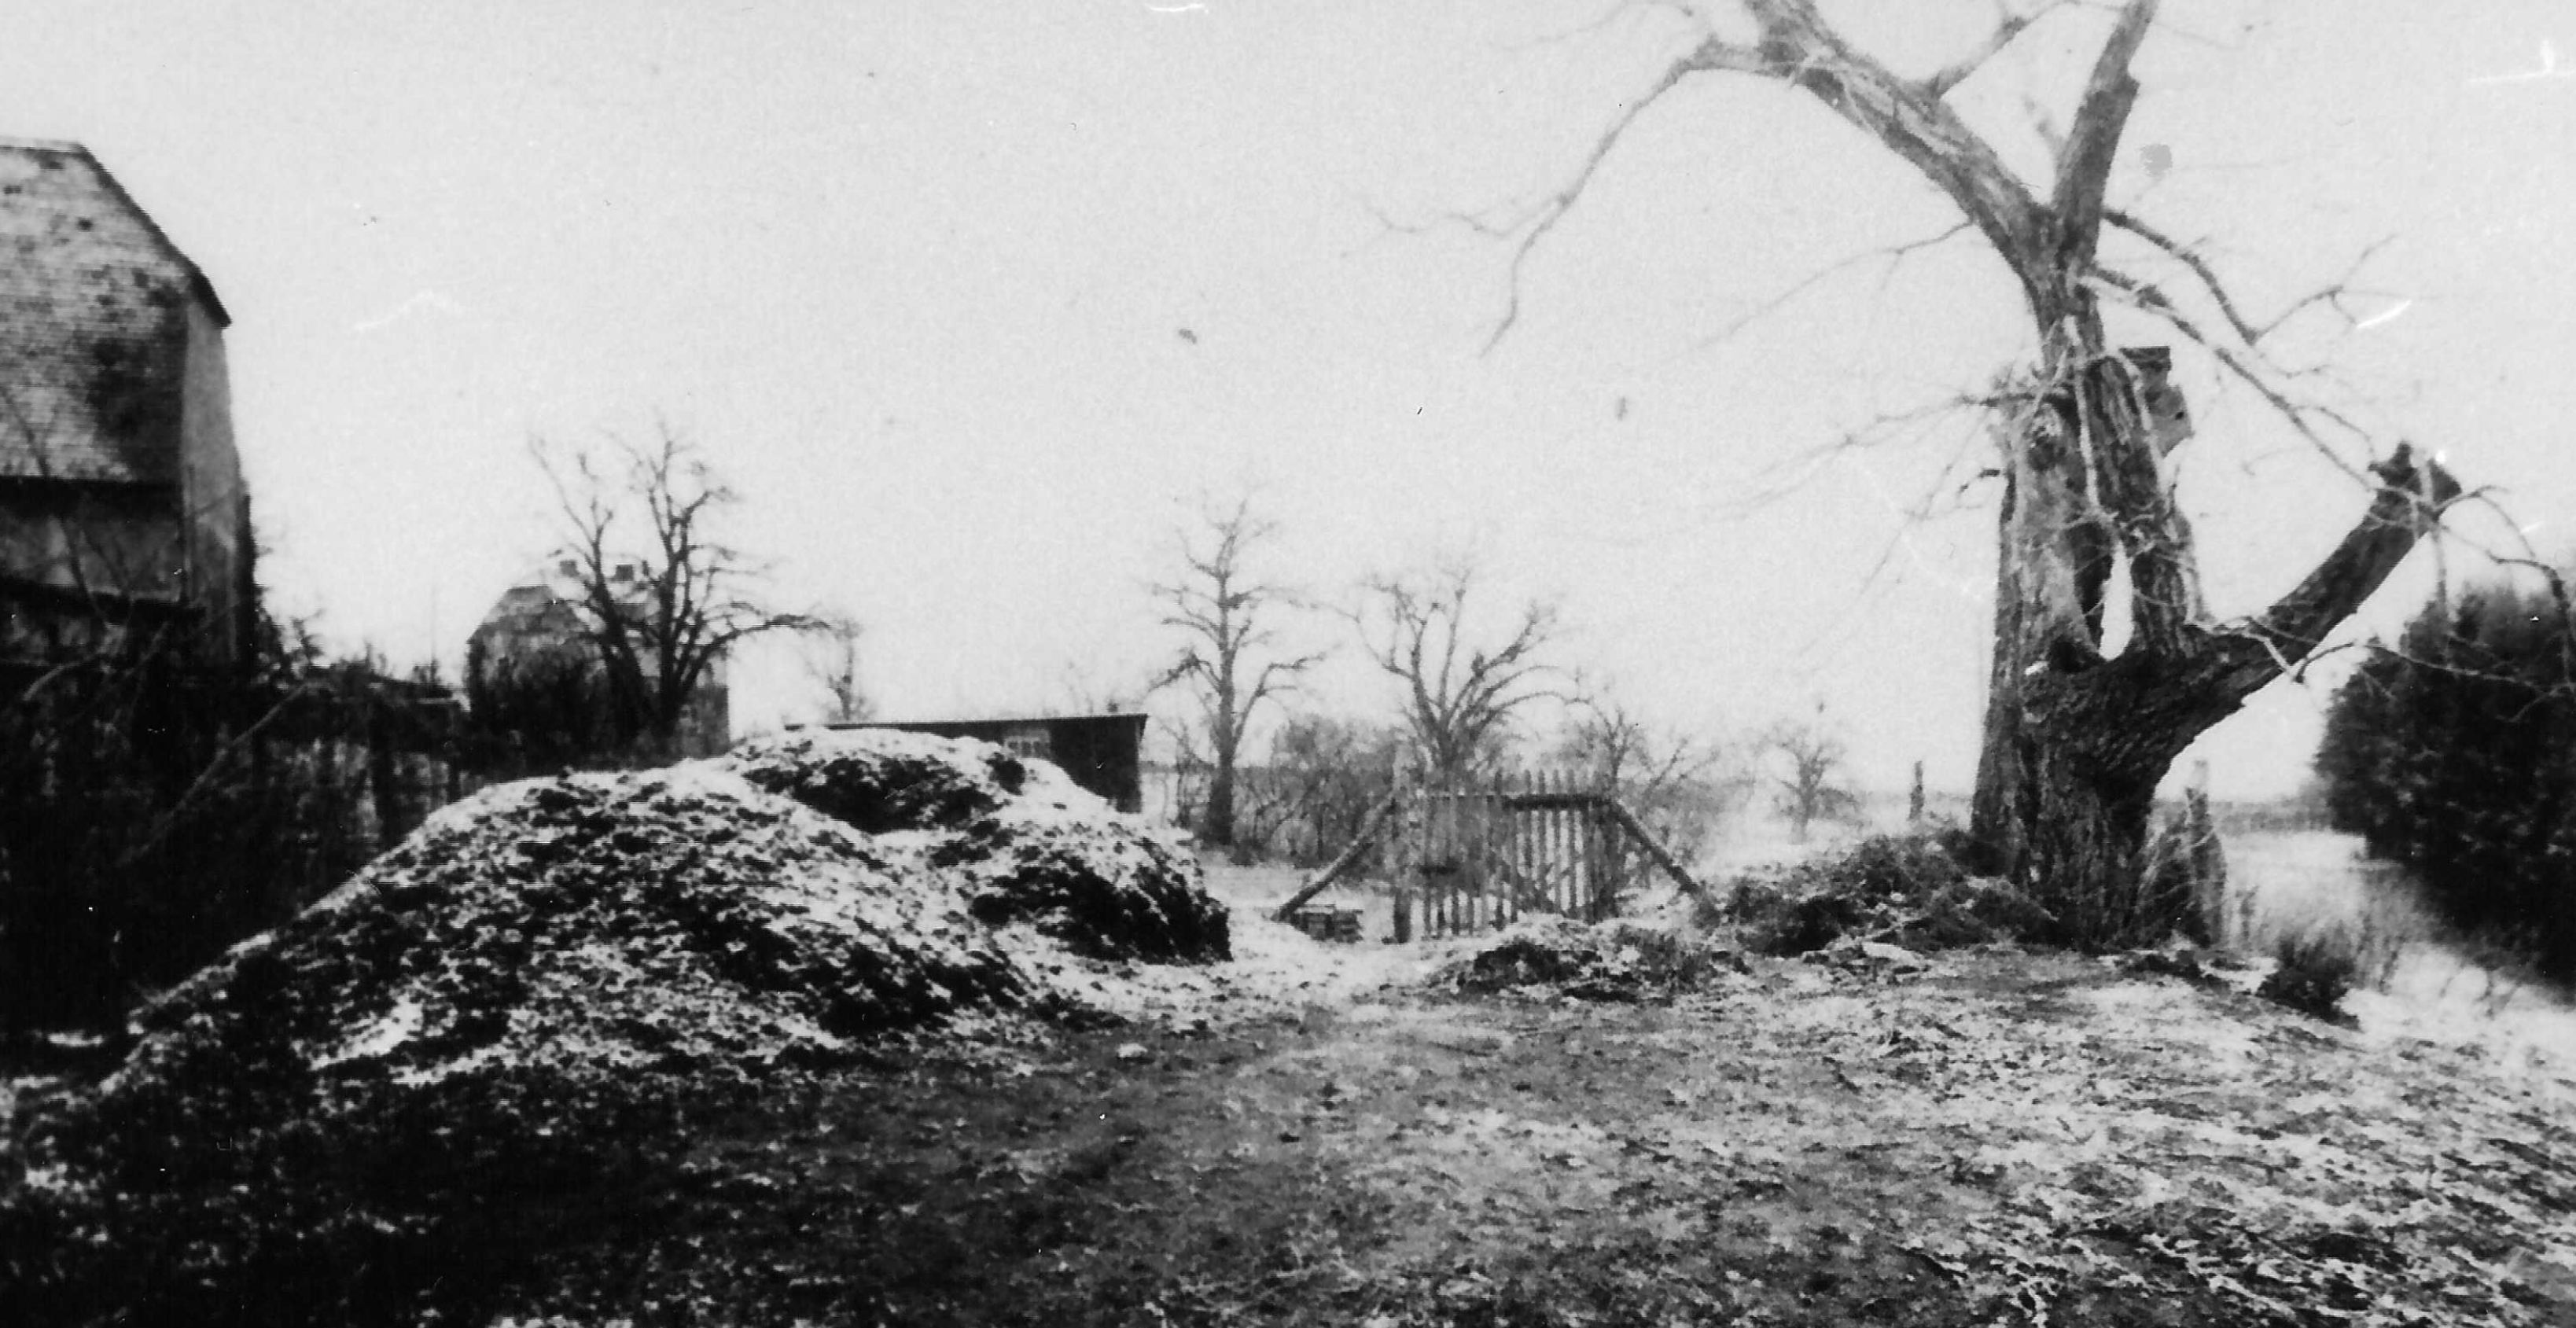
\includegraphics[width=.9\linewidth]{images/tm02}}}\\[-5pt] 

\myfigure{tm03}{BStU MFs Ast StKs 13/48 Bd.2.}{}{}{0.479}\hspace{0pt} 	&

\myfigure{tm04}{BStU MFs Ast StKs 13/48 Bd.2.}{}{}{0.043}		\\[-20pt]
 
\myfigure{tm05}{BStU MFs Ast StKs 13/48 Bd.2.}{}{}{0.479}\hspace{0pt} &

\myfigure{tm06}{BStU MFs Ast StKs 13/48 Bd.2.}{}{}{0.043} \\%[-14pt]



\multicolumn{2}{l}{\setlength{\fboxsep}{0pt}\setlength{\fboxrule}{0pt}
\fbox{\mypics[BStU MFs Ast StKs 13/48 Bd.2.]{\noindent Leichenfunde unter dem Komposthaufen des Stadtguts}{Leichenfunde im Stadtgut Kunnerwitz (Komposthaufen)}}}
\end{tabular}
\setlength{\fboxrule}{1pt}
%%
\newpage

\begin{tabular}{p{.45\linewidth}p{.45\linewidth}}
\myfigure{tm07}{BStU}{}{}{0}		& 
\myfigure{tm08}{BStU}{}{}{0}		\\[-35pt]
\myfigure{tm09}{BStU}{}{}{0}\hspace{-35pt}		&
\myfigure{tm10}{BStU}{}{}{0}		\\[-35pt]
\myfigure{tm11}{BStU}{}{}{0}\hspace{-35pt}		& 
\myfigure{tm12}{BStU}{}{}{0}\\[-20pt]
\multicolumn{2}{l}{\setlength{\fboxsep}{0pt}\setlength{\fboxrule}{0pt}
\fbox{\mypics[BStU MFs Ast StKs 13/48 Bd.2.]{Leichenfunde an der Mauer des Stadtguts}{Leichenfunde im Stadtgut Kunnerwitz (Mauer)}}}
\end{tabular}



%%%%%%%%%%%%%%%%
\paragraph{Deutsch-Paulsdorf\index{o}{Deutsch-Paulsdorf}}
In Deutsch-Paulsdorf\index{o}{Deutsch-Paulsdorf} wurden laut Hinweisen der Bevölkerung insgesamt vier getötete Häftlinge gefunden, deren Verbleib ungewiss ist. Nach Recherchen des damals in der Sache ermittelnden Kriminalkommissars Kurt Wolf\index{p}{Wolf, Kurt} lag ein Toter an der \glqq Waage\grqq~(Waage für landwirtschaftliche Güter), zwei weitere in der Nähe des Hofes von Familie Schmidt\index{p}{Schmidt} und ein Leichnam in der Sandgrube, nahe dem ehemaligen Abzweig nach Altbernsdorf\index{o}{Altbernsdorf}\footnote{Interview mit Kurt Wolf, Löbau 2005-10}.


%%%%%%%%%%%%%%%%
\paragraph{Obersohland am Rotstein\index{o}{Obersohland}\label{sohland}}
Während des Aufenthalts der Gefangenen im Göbelschen\index{p}{Göbel} Gut in Obersohland\index{o}{Obersohland} starben des nachts fünf Menschen; angeblich weil sie versuchten, auf den Dachbalken der Scheune zu schlafen und herunter fielen. Jene fünf Leichen wurden an einem unbekannten Ort hinter dem Obersohländer\index{o}{Obersohland} Friedhof beigesetzt und mit keinem Wort in den Kirchenbüchern vermerkt.
\newline
In einem nahe gelegenen Waldstück kam es angeblich zu einer Erschießung von sieben Menschen. Der genaue Ort ist bis heute unbekannt\footnote{Vgl. Schlomo Graber: Schlajme. Vgl. auch Jakob Rosenbaum: Von Görlitz nach Tirol.}.


%%%%%%%%%%%%%%%%
\paragraph{Lehdehäuser\index{o}{Lehdehäuser}}
Wie bereits erwähnt, waren einige Bewohner der Lehdehäuser\index{o}{Lehdehäuser} Zeuge, wie vor ihren Augen ein entkräfteter Häftling niedergeschlagen und erschossen wurde. Wahrscheinlich sammelte das \glqq Leichenkommando\grqq~den Toten später ein, denn laut Aussage eines Anwohners hinterließ die Gefangenenkolonne keine Spuren. 

%%%%%%%%%%%%%%%%
\paragraph{Buschschenke\label{buschschenke}}
Gerda Bötig bezeugt einen Toten, den sie unweit vom elterlichen Haus auf der Straße liegend fand.
~\newline
Am 03. November 1947 heißt es in einem Polizeibericht, dass man auf der Verbindungsstraße Kemmnitz--Strahwalde sieben Leichen im Wald gefunden hatte (Bild ~\mypicsref{leichenwald}), \glqq welche am 26.02.1945 durch den Totenbettmeister von Kemnitz\index{o}{Kemnitz}, August Hänsch\index{p}{Hänsch, August}, auf Anordnung des damaligen Bürgermeisters von Kemnitz\index{o}{Kemnitz}, Richard Milsch\index{p}{Milsch, Richard}, an der Fundstelle beerdigt wurden.\grqq\footnote{BStU MfS ASt 13/48 Bd. 2 / 479.}. Die Exhumierung im Jahre 1947 geschah im Beisein der Großschweidnitzer Ärzte Dr. Ehrlich\index{p}{Ehrlich, Dr.} und Fräulein Dr. Elfriede Ochsenfahrt\index{p}{Ochsenfahrt, Elfriede Dr.}\footnote{xxx Zusammenhang mit Euthanansieverbechen in Großschweidnitz klären.}. Von den gefundenen sieben stark verwesten Leichen waren drei Schädel total zertrümmert, ein weiterer wies an beiden Schläfen handtellergroße Sprünge auf\footnote{BStU MfS ASt 13/48 Bd. 2 / 481.}. Bei den drei anderen Skeletten konnten die Ärzte keine sichtbaren Spuren von Gewalteinwirkung feststellen. Die Umbettung geschah am 4. November 1947; wohin, wurde nicht erwähnt.
\newline
Ferner gibt der Polizeibericht Aufschluss über die persönlichen Dinge, welche die Opfer während des Marsches mit sich führten. Neben sieben paar Holzschuhen fanden die Ermittler: \glqq 1 Tabakdose mit Inhalt eine Zigarettenspitze, 1 Ausschnitt einer Zeitung in slawischer Sprache, 5 blecherne Essschüsseln, 3 Löffel, 1 Taschenmesser und 2 feststehende Messer\grqq.

\myfigure[leichenwald]{tm13}{BStU MFs Ast StKs 13/48 Bd.2.}{Leichenfunden im Wald zwischen der Buschschenke\index{o}{Buschschenke} und Berthelsdorf\index{o}{Berthelsdorf}}{Leichenfunde im Wald}{0}

Zu den Fundstücken zählte die Polizei noch etwas wesentlich Wertvolleres, dessen sich die damaligen Machthaber in gleicher Weise bedienten, wie zuvor die SS in den Konzentrationslagern:

\begin{leftbar} 
Ferner wurden auf Anordnung der SMA [Sowjetische Militäradministration] die Gold- und Silberzähne aus den Gebissen der Toten entfernt und werden sofort nach Eintreffen in der hiesigen Dienststelle der SMA-Dienststelle Löbau/Sa. zugestellt.\footnote{BStU MfS ASt 13/48 Bd. 2 / 481.}
\end{leftbar} 
Der materielle Wert des Edelmetalls wiegt bei diesem Befehl offensichtlich schwerer als die Pietät.

%%%%%%%%%%%%%%%%
\paragraph{Berthelsdorf\index{o}{Berthelsdorf}}
Es gibt Gerüchte über Leichenfunde zwischen der Neuberthelsdorfer Sandgrube und dem Oberhof (Berthelsdorf\index{o}{Berthelsdorf}), jedoch keine bestätigten Funde\footnote{Laut Hinweisen von Ilse Gießler und Wolfgang Bittrich\index{p}{Bittrich, Wolfgang} sowie einiger anderer Berthelsdorfer\index{o}{Berthelsdorf} Bürger.}. Alle innerhalb der Ortschaft verstorbenen Menschen schaffte man wahrscheinlich mittels Wagen nach Rennersdorf\footnote{Hildegard Fleischmann. BStU MfS ASt 13/48 Bd. 2 / 460.}.


%%%%%%%%%%%%%%%%%%%%%%%%%%%%%%%%%%%%%%%%%%%
\subsubsection{Opfer in Rennersdorf}
Die Zahl der in Rennersdorf zu Tode gekommenen KZ-Gefangenen ist ebenso unbestimmt wie die Opferzahl während des Todesmarsches. 

Laut dem damaligen Ortschronisten Robert Heinze\index{p}{Heinze, Robert} wurden bereits im Oktober 1945 insgesamt acht Leichen durch ehemalige Rennersdorfer NSDAP-Mitglieder freigelegt und auf den örtlichen Friedhof umgebettet\footnote{Robert Heinze: Ortschronik Rennersdorf. Dies stimmt mit der Aussage von Christa Schubert überein, deren Vater der Ausgrabungsaktion beiwohnen musste.}. Bei der Exhumierung verpflichtete die SMA eine Schulklasse aus Rennersdorf zur Anwesenheit\footnote{Aussage von Christa Schubert, deren Bruder im Kindesalter bei den Ausgrabungen anwesend war.}.

Eine andere Rennersdorfer Schulklasse machte bei einem Ausflug eine grausige Entdeckung, als beim Laufen abseits des Weges mehrere Knochen hervortraten\footnote{Edeltraud Bittrich. Interview vom 29.03.2004.}. Die daraufhin verständigte Polizei leitete weitere Ermittlungen ein.
Am Donnerstag dem 29.01.1948 kam es dann in Rennersdorf zur Ausgrabung von vier Leichen. Anwesend waren der Polizeiarzt Dr. Gottschalk\index{p}{Gottschalk, Dr.} aus Görlitz und die Kriminalkommissare Reimann\index{p}{Reimann (Kommisar)}, Wolf\index{p}{Wolf, Kurt}, Hulek\index{p}{Hulek (Kriminaltechniker)}, der stellvertretende Bürgermeister Richter\index{p}{Richter}\footnote{BStU MfS ASt 13/48 Bd. 2 / 465.}, ferner einige Arbeiter, zumeist ehemalige Mitglieder der Hitlerjugend\footnote{Laut Günter Scholze, der damals selbst mit Hand anlegen musste. Telefonisches Interview vom 29.03.2004.}.
\begin{leftbar} 
An einem etwa 2 Meter hohen Abhang befand sich die Fundstelle. Der Abhang war mit Grasbüschen bewachsen. Die Fundstelle war bei unserem Eintreffen leicht mit Erde und Stroh zugedeckt. Die Kriminalpolizei hatte bereits einige Tage zuvor mit dem Suchen begonnen. Als sie dabei auf die Knochenreste stießen, wurde die Arbeit nicht fortgesetzt, da die Kriminaldienststelle Görlitz K5 verständigt werden musste\footnote{Das erklärt, warum die Fundstelle mit Stroh und Erde abgedeckt war.}.
\newline
Nachdem von uns die Erde entfernt wurde, waren 4 Skelette von Leichen zu sehen, die in schwarze Lumpen gehüllt waren. Die Skelette lagen geschichtet nebeneinander, zwei Kopfschädel neben den Beinen und Fußknochen der beiden anderen Skelette, die in umgekehrter Richtung lagen. Beim Herausnehmen der Knochenstücke zerfielen diese sofort in einzelne Stücke, so dass der Zusammenhang verloren ging. Bei der oberflächlichen Untersuchung durch Dr. Gott-schalk\index{p}{Gottschalk, Dr.} konnten keine Schuss- oder Schlagverletzungen festgestellt werden. Die Knochenstücke wurden in Papiersäcke geborgen und im Kraftwagen nach Görlitz gebracht.\footnote{BStU MfS ASt 13/48 Bd. 2 / 465.}
\end{leftbar}
Merkwürdig erschien den Ärzten, dass sämtliche Schädel Frakturen mit glatten geradlinigen Bruchlinien aufwiesen, die eine Einwirkung eines stumpfen Gegenstandes ausschließen\footnote{BStU MfS ASt 13/48 Bd. 2 / 467.}.
Bei zwei der Leichen fehlten die Halswirbel (Atlas), was auf einen Einschuss im Genick als Todesursache schließen läßt. 
\newline
Der Verbleib dieser insgesamt zwölf Leichname in Rennersdorf ist indes nur teilweise geklärt. Laut der Grabsteininschrift sind auf dem Rennersdorfer Friedhof 10 jüdische Menschen begraben. Demnach bestattete man neben den acht, im Jahre 1945 gefundenen, Leichen, noch zwei weitere, deren Fundstelle unbekannt ist oder mit der im Februar 1948 aufgedeckten Grabstätte übereinstimmt (siehe auch S.~\pageref{leichen}).

Die Differenz zwischen den von Emmrich Schiffer dokumentierten 75 in Rennersdorf angekommenen Toten und den tatsächlich gefundenen 12 Leichnamen, konnte nicht aufgeklärt werden. Auch die im Jahre 2010 im Auftrag des Sächsischen Landesamtes für Archäologie durchgeführten archäologischen Untersuchungen des Waldstücks neben dem Pferdestall blieben ergebnislos.

%%%%%%%%%%%%%%%%%%%%%%%%%%%%%%%%%%%%%%%%%%%
\subsubsection{Todesopfer zwischen März und Mai 1945}

Bei Rückkehr der Gefangenen nach Görlitz befand sich die Stadt immer noch im Ausnahmezustand. Die Flüchtlingsströme aus Osten und die nahe liegende Front bedingten während dieser Zeit viele Todesfälle, welche die örtlichen Bestatter kaum noch bewältigen konnten. 
Im Tagebucheintrag des Görlitzer Predigers Franz Scholz\index{p}{Scholz, Franz}\footnote{Franz Scholz wurde später wegen seines couragierten Eintretens für Kriegsgefangene zum Ehrenbürger der Stadt Görlitz ernannt.} heißt es bereits am 12. Februar:
\begin{leftbar}
Die Leichenhalle auf dem städtischen Zentralfriedhof platzt aus allen Nähten. Die Toten sind dort längst nicht mehr alle unterzubringen. [...] Für die Leichen der Erwachsenen wird die riesige Halle der Nikolaikirche bestimmt.
\end{leftbar}
\newpage
Es scheint klar, dass die Einäscherung weiterer KZ-Häftlinge unter diesen Umständen unmöglich erschien\footnote{Einige Quellen berichten zudem vom Ausfall der Gasversorgung im Krematorium, dies konnte jedoch nicht weiter bestätigt werden.} und die Lagerleitung eine andere Möglichkeit finden musste, sich der fortlaufenden Todesopfer im Lager zu entledigen.
\newline
Berichte, wonach es auch im Krematorium Zittau zur Einäscherung Görlitzer Häftlinge kam, ließen sich weder widerlegen noch eindeutig bestätigen. Im Krematorium Zittau\index{o}{Zittau} sind zwischen dem 19. Februar und 7. Mai 1945 insgesamt 106 jüdische Häftlinge in den Einäscherungsbüchern verzeichnet. Mindestens 29 der dort aufgeführten Häftlingsnummern weichen nur geringfügig von den Nummern Görlitzer Häftlinge ab. Die Angaben sind aber jeweils nicht eindeutig einer Person zuzuordnen, da entweder die Häftlingsnummer oder der Name gelistet ist.
\newline
Der nur wenige hundert Meter vom Lager entfernte Jüdischen Friedhof wurde in der folgenden Zeit als notdürftiger Bestattungsort der toten Häftlinge sowie der im Lager hingerichteten Personen genutzt. Die Gefangenen mussten dafür mehrere Massengräber errichten. 
\newline
Zur Öffnung zweier Massengräber auf dem jüdischen Friedhof kam es zwischen dem 19. und 22. Februar 1948 im Zuge der Ermittlungen gegen den Görlitzer Kreisleiter Malitz\index{p}{Malitz, Dr. Bruno} und Oberbürgermeisters Meinshausen\index{p}{Meinshausen, Dr. Hans}\footnote{Laut Aussage von Kurt Wolf, welcher damals zusammen mit Kommissar Mellmann die Ausgrabungen auf dem Jüdischen Friedhof leitete. Interviews mit Kurt Wolf, Löbau 2005-10.}. 
Bei der gleichzeitigen Exhumierung der sterblichen Überreste fanden die Ermittler insgesamt 173 Leichen (Bild.~\ref{leichenzeitung}), darunter sechs Särge mit jeweils 1--3 Leichen darin. Alle übrigen Leichen fanden die Ermittler in bis zu vier Schichten übereinander gestapelt und unbekleidet in den Gräbern. Mindestens\label{weiss} drei von ihnen hatten längere Haare, was zunächst die Vermutung nahe legt, dass es sich bei ihnen nicht um Lagerinsassen handelt, sondern vielmehr um die Kriegsgefangenen, die während der letzten beiden Kriegsmonate im Lager umgebracht wurden. Dieser Schluss gilt nicht unbedingt, da insbesondere jene Frauen im Lager lange Haar trugen, die ab Januar 1945 in Görlitz eintrafen\footnote{Interview mit Anna Hyndr\'akov\'a, Prag 2005.}. 

Als bemerkenswert gilt der Fund von einer in weißes Tuch gehüllten Frau. Der Überlebende Janek Oborowicz\index{p}{Oborowicz, Janusch} bekundet, dass es sich dabei um eine Ungarin handelt, deren Leichnam er selbst gesehen hat\footnote{\glqq Der Rapportführer sagte, dass vor einigen Tagen eine Ungarin beigesetzt wurde.\grqq~Janek Oborowicz. BStU MfS ASt 13/48 Bd. 2 / 472.}. Darüber hinaus konnten die Ermittler unter den Opfern noch zwei weitere Frauen ausmachen. Einige Leichen trugen Zivilkleidung und bei zwei weiteren konnte eindeutig festgestellt werden, dass sie zum Zeitpunkt des Todes nicht älter als 19 bzw. 20 Jahre waren.
Die Polizei\linebreak\newpage stellte schließlich fest, dass einige (nicht unbedingt alle) der im Lager von der SS und Gestapo hingerichteten Kriegsgefangenen und Fremdarbeiter an keinem anderen Ort als dem Jüdischen Friedhof beigesetzt wurden\footnote{Juda Widawski. LArchB B Rep 058 Bd. 2. Siehe auch BStU MfS ASt 13/48 Bd. 2 / 549.}.
~\newline
Der damals in die Ermittlungen involvierte Polizeikommissar Kurt Wolf\index{p}{Wolf, Kurt} schreibt dazu:
\begin{leftbar}
Oberarzt Dr. Scheit\index{p}{Scheit, Dr.} vom Friedrichstädter Krankenhaus in Dresden\index{o}{Dresden} konnte anhand von Ein- und Ausschusslöchern oder Schlagverletzungen am Kopf nachweisen, dass ein großer Teil der Häftlinge nicht nur eines Hungertodes starb, sondern durch äußere und brutale Gewalteinwirkung.\footnote{Kurt Wolf: Das KZ-Außenlager Görlitz Biesnitzer Grund, S. 23.}
\end{leftbar}

\myfigure[leichenzeitung]{YV-1948-ExhumierungJuedischerFriedhof.png}{YV 951, Id: 52982.}{Presseecho zu den Leichenfunden auf dem Jüdischen Friedhof.}{Presseecho zu den Leichenfunden auf dem Jüdischen Friedhof.}{0}

%%%%%%%%%%%%%%%%%%
%% Fotos der Leichenfunde auf dem juedischen Friedhof
\hspace{-8pt}
\begin{tabular}{p{.305\linewidth}p{.305\linewidth}p{.305\linewidth}}
\myfigure{jf_schaedel_3}{}{}{Jüdischer Friedhof: Schädel}{0}&
\myfigure{jf_schaedel_1}{}{}{Jüdischer Friedhof: Schädel}{0}&
\myfigure{jf_schaedel_2}{}{}{Jüdischer Friedhof: Schädel}{0}
\\[-14pt]
\multicolumn{3}{l}{\setlength{\fboxsep}{0pt}\setlength{\fboxrule}{0pt}
\mypics[BStU MFs Ast StKs 13/48 Bd.2.]{Ein zertrümmerter und zwei Schädel mit Einschussloch}{Schädelfunde auf dem Jüdischen Friedhof}}
\end{tabular}

\myfigure{jf02}{BStU MFs Ast StKs 13/48 Bd.2.}{Dr. Scheit\index{p}{Scheit, Dr.} bei der Untersuchung eines Schädels}{Jüdischer Friedhof: Dr. Scheit}{0}

\newpage
\myfigure{jf03}{BStU MFs Ast StKs 13/48 Bd.2.}{Durch Bretter abgetrenntes Massengrab}{}{0}

\myfigure{jf01}{}{Kurt Wolf (zweite v. links) mit Meinshausen\index{p}{Meinshausen, Dr. Hans} (links) und Malitz\index{p}{Malitz, Dr. Bruno} (dritte v. rechts) vor Ort.}{Jüdischer Friedhof: Angeklagte vor Ort}{0}

\myfigure{jf04}{BStU MFs Ast StKs 13/48 Bd.2.}{}{Jüdischer Friedhof: Ausgrabungen}{0}


\myfigure{jf05}{BStU MFs Ast StKs 13/48 Bd.2.}{}{Jüdischer Friedhof: Ausgrabungen}{0}

\myfigure{jf06}{BStU MFs Ast StKs 13/48 Bd.2.}{}{Jüdischer Friedhof: Ausgrabungen}{0}


\myfigure{jf07}{BStU MFs Ast StKs 13/48 Bd.2.}{}{Jüdischer Friedhof: Ausgrabungen}{0}

\myfigure{jf08}{BStU MFs Ast StKs 13/48 Bd.2.}{}{Jüdischer Friedhof: Ausgrabungen}{0}

\myfigure[BStU MFs Ast StKs 13/48 Bd.2.]{jf09}{BStU}{Umbettung der Toten in den hinteren Teil des Friedhofs}{Jüdischer Friedhof: Umbettung}{0}

%%%%%%%%%%%%%%%%%%%%

\newpage
%%%%%%%%%%%%%%%%%%%%%%%%%%%%%%%%%%%%%%%%%%%%%
\section{Ermittlungen gegen NS-Verbrecher\label{ns-verbrechen}}
Bereits im Februar 1942 beschlossen die Alliierten auf der Konferenz von Jalta\index{o}{Jalta}, alles Mögliche zu tun, um \glqq den deutschen Militarismus und Nazismus zu vernichten und endgültig die Garantie dafür zu schaffen, dass Deutschland nie wieder dazu in der Lage sein wird, den Weltfrieden zu brechen\grqq\footnote{Vgl. Peter Reichel: Vergangenheitsbewältigung in Deutschland, S. 30. Siehe auch: Alexander Fischer (Hg.): Teheran -- Jalta -- Potsdam. Die sowjetischen Protokolle von den Kriegskonferenzen der Großen Drei, S. 184f.}. Konkretisiert wurde dieses Vorhaben durch die Direktive Nr. 24 des Alliierten Kontrollrates im Januar 1946.
Um dieses Ziel zu erreichen, sollten alle nazistischen und militärischen Einflüsse aus öffentlichen Einrichtungen, dem Kultur- und Wirtschaftsleben entfernt, und sämtliche Kriegsverbrecher angeklagt und verurteilt werden.
Die Notwendigkeit, die Straftäter des KZ-Außenlagers Görlitz vor Gericht zu stellen, wurde aber auch maßgeblich durch die ehemaligen Gefangenen forciert. Des Weiteren bestand ein erhebliches öffentliches Interesse, die zahlreichen Leichenfunde aufzuklären und die dafür verantwortlichen Personen zur Rechenschaft zu ziehen. 
In der sowjetischen Besatzungszone begannen die Ermittlungen im Zusammenhang mit dem Görlitzer KZ-Lager zwar relativ zeitig, doch ermittelte man erst im Jahre 1948 intensiver, als es darum ging, die Görlitzer \glqq Hauptkriegsverbrecher\grqq~dingfest zu machen. 
Sämtliche Ermittlungsverfahren, die in den westlichen Besatzungszonen bzw. der BRD eingeleitet wurden, basierten entweder auf Strafanzeigen ehemaliger Gefangener oder auf Hinweise polnischer Behörden, welche ihrerseits sehr konsequent gegen NS-Verbrecher vorgingen.
~\newline
Eine vergleichende Bewertung des Umgangs mit NS-Verbrechern in der DDR und der BRD lässt sich anhand der wenigen hier betrachteten Fälle jedoch nicht vornehmen und ist auch nicht das Anliegen dieses Buches. Die hier betrachteten Fälle machen dennoch deutlich, dass die Verantwortung für die Geschehnisse im KZ-Außenlager Görlitz nicht auf eine homogene Personengruppe reduziert werden kann, obwohl weder Staatsanwaltschaften noch Gerichte gewillt waren die Verstrickung zwischen Funktionshäftlingen, Lagerpersonal, Staatsorganen und Wirtschaft gebührend zu berücksichtigen. Dem entgegen steht die wahrscheinlich größere Zahl derer, die von den sowjetischen Besatzern wegen bestimmter Beziehung zum Görlitzer KZ-System ohne richterliches Urteil in sowjetischen Speziallagern wie Bautzen festgehalten wurden\footnote{Hinweis darauf geben Berichte über den Rennersdorfer Gutsverwalter Lehmann, den Fuhrparkleiter Anton Sedlak (Akten sind verschollen) sowie Männer des Wachpersonals. Vgl. BStU MfS ASt 13/48.}. 

Eine genauere Betrachtung der Ermittlungen im Zusammenhang mit dem KZ-Außenlager Görlitz erfolgt anhand der einzelnen Fälle. 

\newpage
%%%%%%
\paragraph{Der Lagerkommandant Erich Rechenberg\index{p}{Rechenberg, Erich}\label{rechenberg_ahndung}}
Die Flucht Rechenberg\index{p}{Rechenberg, Erich}s misslang am 11. Mai 1945 in Deutsch-Gabel\index{o}{Deutsch-Gabel} (Jablonné v Podještědí, Tschechien), wo er und einige Wachleute in die Arme der Roten Armee fielen. Rechenberg\index{p}{Rechenberg, Erich}
verbrachte die folgenden achteinhalb Jahre in den sowjetischen Kriegsgefangenenlagern
Hoyerswerda\index{o}{Hoyerswerda}, Frankfurt/Oder\index{o}{Frankfurt/Oder}, Rybinsk\index{o}{Rybinsk} (ab Juli 1945), Nowo Tscherkask\index{o}{Nowo Tscherkask}, Tanganrok\index{o}{Tanganrok}, Rostow\index{o}{Rostow}, Schachty\index{o}{Schachty}, Tanganrok\index{o}{Tanganrok} und zuletzt in Krasnopolje\index{o}{Krasnopolje} (bis September 1953)\footnote{LArchB B Rep 058 Bd. 2.}. Nach
seiner Rückkehr erhielt er durch die Bundesrepublik Deutschland, offenbar ganz selbstverständlich, 4140 DM Entschädigung für die Zeit seiner Gefangenschaft\footnote{Ebenda.}.
\newline
Nachdem polnische Behörden erhebliches Beweismaterial zur Verfügung stellten, begann die Staatsanwaltschaft Berlin\index{o}{Berlin} im Jahre 1970 gegen Erich Rechenberg\index{p}{Rechenberg, Erich} zu ermitteln.
Gemäß \S\,170 Abs.~2 wurde das Verfahren gegen ihn am 6. Dezember 1971 aufgrund widersprüchlicher Zeugenaussagen und fehlender Identifizierung der Person Rechenberg\index{p}{Rechenberg, Erich} durch Zeugen eingestellt. Der Name Rechenberg\index{p}{Rechenberg, Erich} war den über 100 Befragten zumeist unbekannt, nicht jedoch sein Aussehen. Bei den Rechthilfeersuchen verzichteten die Behörden auf die Beilegung von Fotos des Beschuldigten und fragten statt dessen nur nach seinem Namen. Letztlich fand sich lediglich ein belastender Zeuge, dessen alleinige Aussage allerdings nicht als ausreichend erachtet wurde und zudem teilweise im Widerspruch zu Aussagen anderer Häftlinge stand. Während des gesamten Verfahrens wurde Rechenberg\index{p}{Rechenberg, Erich} nicht ein einziges Mal zu den Vorwürfen befragt. Die Polizei tat sich sogar schwer, Herrn Rechenberg\index{p}{Rechenberg, Erich} daheim ausfindig zu machen, obwohl er seinen Wohnsitz seit den 1950er Jahren nicht änderte und zeitweilig sogar eine Anstellung im Landgericht Berlin\index{o}{Berlin} hatte. Die ermittelnde Staatsanwaltschaft versäumte es völlig, in Betracht zu ziehen, dass sich Rechenberg\index{p}{Rechenberg, Erich}s Verantwortungsbereich auf fünf weitere KZ-Außenlagern erstreckte, deren Überlebende nicht zu Aussagen herangezogen wurden.
~\newline
Aber was zählt schon ein Überlebender. Der Berliner\index{o}{Berlin} Oberstaatsanwalt Wolke\index{p}{Wolke} brachte es letztmalig am 20. August 1996 in einer Verfügung auf den Punkt:
\begin{leftbar} 
Was der Zeuge Schlomo Graber\index{p}{Graber, Schlomo} in Bezug auf den Beschuldigten sagen kann, ist nicht bekannt. Es dürfte kaum damit zu rechnen sein, dass er Umstände zu bekunden in der Lage ist, die zu einer Wiederaufnahme des Verfahrens führen. Dessen ungeachtet wird man wohl den Versuch machen müssen, ihn zu hören. Da die Anhörung nach Lage der Dinge sich aber nicht auf konkrete, in das Wissen des Zeugen gestellte Tatsachen stützt, sondern nur darauf beruht, dass er Überlebender des KL ist, dürfte eine förmliche Wiederaufnahme der Ermittlungen damit nicht verbunden sein.\footnote{LArchB B Rep 058 Bd. 11.}
\end{leftbar}
\newpage
Um bei Herrn Wolke\index{p}{Wolke} Gehör zu finden, bedarf es offenbar etwas mehr als das Bezeugen von Straftaten. Schlomo Graber\index{p}{Graber, Schlomo} wurde nie von deutschen Behörden zu den Verbrechen im KZ-Außenlager Görlitz befragt. Erich Rechenberg\index{p}{Rechenberg, Erich} erfreute sich eines hohen Alters und verstarb im Jahre 2000 in Ratzeburg bei Berlin\index{o}{Berlin}.


%%%%%%%%%%
\paragraph{Lagerführer Zunker\label{zunker_ahndung}}
Über das Schicksal des Oberscharführers Zunker ist nur soviel sicher, dass er nach einer Kriegsgefangenschaft in Dachau 1947 an Polen ausgeliefert und am 25. Januar 1949, zusammen mit dem Lagerältesten Czech, in \L \'od\'z hingerichtet wurde\footnote{Prozess gegen Winfried Zunker, Az.: VII K 1613/48, VII 1614/48. Kriegsgericht \L \'od\'z.}.
Gerüchten nach war Zunker mit einer ungarischen Jüdin liiert und hat sich gemeinsam mit ihr auf die Flucht begeben\footnote{Laut Anna Hyndr\'akov\'a, die mit ihm flüchtete.}.




%%%%%%%%%%%%%%%%%%%%%%%%
\paragraph{Der Lagerälteste Hermann Czech\index{p}{Czech, Hermann}\label{czech_ahndung}} 
Ein ehemaliger Häftling des KZ-Außenlagers Bunzlau\index{o}{Bunzlau} (heute: Boles\l awiec, Polen) namens Monik Mlynarski\index{p}{Mlynarski, Monik} verbrachte während der Evakuierung seines Lagers zwar nur wenige Tage im Görlitzer Lager, doch gelang es ihm den Görlitzer Lagerälteste ausfindig zu machen:
\begin{leftbar} 
Ich wollte ein Schloss in einem Erfurter\index{o}{Erfurt} Eisenwarengeschäft kaufen. Dies war nicht zu haben, deshalb wollte ich den Chef sprechen. Dieser war Czech\index{p}{Czech, Hermann}. Ich fragte, ob er Lagerältester in Görlitz gewesen sei. Er erwiderte: \glqq Alter Kollege\grqq~und bot mir eine Zigarette an. Im Hotel erzählte ich meinen Freunden davon. Diese wiederum klärten mich auf, dass Czech\index{p}{Czech, Hermann} der schlimmste Verbrecher sei und Frauen vergewaltigt hatte. Daraufhin habe ich Czech\index{p}{Czech, Hermann} bei der Polizei angezeigt.\footnote{Telefonisches Interview mit Monik Mlynarski vom 18.11.2004.}
\end{leftbar}

Ein von ehemaligen Häftlingen aufgesetztes Schreiben führte 1947 zur Verhaftung Hermann Czech\index{p}{Czech, Hermann}s:

\begin{leftbar}Berlin-Schlachtensee\index{o}{Berlin}, 22. Februar 1947:\\ 
Die unterzeichneten ehemaligen KZ-Häftlinge des KZ-Lagers Görlitz bitten die Behörden hiermit, die Verhaftung des\newline
Hermann C Z E C H\index{p}{Czech, Hermann}\\
geb. 27.10.1892\\ 
in Breslau\\
jetzt Wohnhaft in Erfurt\index{o}{Erfurt}, Zeitlitzerstr. 12, b/Herrn Zenser vorzunehmen.\newline
Dieser Hermann Czech\index{p}{Czech, Hermann} war im KZ-Lager Görlitz bis März 1945 als Berufsverbrecher Lagerältester. In dieser Eigenschaft hat er alles getan, um die Häftlinge für jede Kleinigkeit zu quälen und zu ermorden. Er hat beim Lagerkommandanten die Erschießung von unzähligen Häftlingen veranlasst. Er selbst hat täglich die Häftlinge für jede Kleinigkeit durchgepeitscht und gequält, hat das Essen, was für Lagerinsassen bestimmt war, für eigene Zwecke und für seine Leute genommen. Sein Vermögen hat er durch Diebstahl von Kleidern, Lebensmitteln, sowie Zigaretten, die für die Häftlinge bestimmt waren, erworben. Er war der grausamste Sadist, der seine Freude an der Quälerei und Ermordung der Häftlinge hatte. Kranke Häftlinge hat er aus dem Revier genommen und sie zur Arbeit gejagt, von der sie nicht mehr zurück kamen. Dagegen hat er seine Kapos und Mithelfer geschützt und sie damit zu weiteren Schandtaten angespornt. Die Zuteilung von Lebensmitteln und Zigaretten, welche die Häftlinge für ihre Arbeit von der Firma WUMAG bekommen sollten, hat er verschoben und die Häftlinge verhungern lassen.\footnote{PMGR 70/4593/MF.}
\end{leftbar}
Izaak Weintraub\index{p}{Weintraub, Izaak}, Bernard Rus\index{p}{Rus, Bernard} und Leon Hecht\index{p}{Hecht, Leon} veranlassten durch ihre Aussagen bei der Polish War Crimes Mission in Bad Salzuflen\index{o}{Bad Sulzuflen} einen Auslieferungsantrag nach Polen. Am 20.7.1947 wurde er schließlich dorthin ausgeliefert und 1948 zusammen mit dem ehemaligen SS-Lagerfüher Zunker vor dem Kriegsgericht in \L \'od\'z\index{o}{\L \'od\'z} zum Tode verurteilt\footnote{Prozess gegen Hermann Czech\index{p}{Czech, Hermann}, Az.: VII K 1613/48, VII 1614/48. Kriegsgericht \L \'od\'z.}.
Die Vollstreckung des Urteils erfolgte am 27. Januar 1949.

%%%%%%%%%%%%%%%%%%%
\paragraph{Die Lagerkapos\label{kapos_ahndung}}
Einen Tag vor der Befreiung des Lagers hatte sich der Lagerkapo Jacob Tannenbaum nach Italien abgesetzt, wo er mit importierten Schwarzmarktgütern Geschäfte machte. In Florenz lernte er seine zweite, 20 Jahre jüngere Frau kennen, mit der er später drei Kinder hatte. Der \emph{Displaced Persons Act} ermöglichte Tannenbaum\index{p}{Tannenbaum, Jacob} im Dezember 1949 die Einreise in die USA. Sechs Jahre später, im März 1955, erkannte man ihm die amerikanische Staatsbürgerschaft zu\footnote{Bekanntgabe des \glqq United States Department of Justice\grqq~vom 12. Mai 1987.}. 
In New York arbeitete er in der Folgezeit bei einem Lebensmittelgroßhändler. Seine aktive Mitgliedschaft in der orthodoxen Jüdischen Gemeinde \emph{Temple Beth El} in Manhattan Beach verlieh ihm Anonymität, da ihre Mitglieder von den übrigen orthodoxen Gemeinden relativ isoliert waren.\newline

Nachdem die USA über 35 Jahre lang Kriegsverbrecher in der Mitte der Gesellschaft ignoriert hat, gründete das Justizministerium 1979 das \emph{Office of Special Investigations} (OSI). Dieses befasste sich mit Tannenbaum, welcher 1978 duch einen ehemaligen Görlitzer Häftling angezeigt wurde. Der Fall verzögerten sich jedoch bis in die späten 1980er Jahre aufgrund der außergewöhnlichen ethischen Komplexität, den Schwierigkeiten an dutzende Zeugenaussagen aus aller Welt zu gelangen und den Vorgesetzten, die sich schwer damit taten, einen Juden eines Kriegsverbrechens anzuklagen. Ihm wurde vorgeworfen, als Aufseher in einem NS-Konzentrationslager an der Verfolgung und Inhaftierung von Menschen, aufgrund ihrer Rasse oder Religion, beteiligt gewesen zu sein. In der Pressemeldung des OSI werden Tannenbaum brutale körperliche Misshandlungen an Häftlingen vorgeworfen. Es handelte sich um einen Zivil-, nicht jedoch um ein Strafprozess, bei dem es darum ging, Tannenbaum auszubürgern und abzuschieben. Während der Verhöre durch die beteiligten Anwälte verlor Tannenbaum mehrmals das Bewusstsein. Ärzte attestierten ihm Herz- und Kreislaufbeschwerden. Angesichts seiner gesundheitlichen Verfassung ersuchte man, um seines Lebens Willen, keine Abschiebung. Die US-Regierung beließ es dabei, da Tannenbaum seine staatsbürgerlichen Rechte, d.h. seine US-amerikanische Staatsbürgerschaft freiwillig abgab. In ähnlichen Fällen hatten die USA bereits John Demjanjuk\index{p}{Demjanjuk, John} nach Israel und Karl Linnas\index{p}{Linnas, Karl} an die UDSSR ausgewiesen. Tannenbaum hätte ein ähnliches Schicksal ereilt, wenn man ihn unmittelbar nach der Anzeige des Falls -- als er sich noch bester Gesundheit wägte --  verurteilt hätte
Der ambivalente Fall Tannenbaum\index{p}{Tannenbaum, Jacob} erregte internationales Aufsehen in den Medien und bei jüdischen Organisationen\footnote{Ebenda. Vgl. auch: Schlomo Graber: Schlajme, S. 82. Der Konflikt wurde 2003 von Jeffrey Sweet im Theaterstück \glqq The Action Against Sol Schumann\grqq~thematisiert und am \emph{Victory Gardens Theatre} Chicago uraufgeführt.}. Tannenbaum spendete Zeit seines Lebens an das \emph{Simon Wiesenthal Center} in Los Angeles.\footnote{David van Biema: Poisoned Lives.} 
~\newline
Der zweite Lagerkapo, Schneebaum\index{p}{Schneebaum}, soll unter anderen Namen in den USA untergetaucht sein.


% In einem Artikel der Süddeutschen Zeitung vom 4. Mai 1987 heißt es:\begin{leftbar} Das Justizministerium arbeitet an der Ausweisung des 75 Jahre alten orthodoxen Juden Jacob Tannenbaum\index{p}{Tannenbaum, Jacob}, der während des Krieges als Aufseher aus den Reihen der Häftlinge im Arbeitslager Görlitz Mithäftlinge geschlagen und gequält haben soll. Das berichten Kreise des Ministeriums in Washington. Tannenbaum\index{p}{Tannenbaum, Jacob}, der die gegen ihn erhobenen Vorwürfe bestreitet und seine Frau, ein Neugeborenes, Vater, Mutter und fünf Schwestern in Konzentrationslagern verloren hat, lebt seit 1949 in New York\index{o}{New York}. 1955 bekam er die amerikanische Staatsbürgerschaft. Nach Angaben des Justizministerium wird seit 1970 gegen ihn ermittelt. Die israelische Regierung habe zahlreiche Informationen zu dem Fall geliefert und auch Belastungszeugen genannt.\footnote{RAG Sammlungsgut KZ Biesnitzer Grund. Ein solcher Artikel erschienen durch eine dpa-Meldung in vielen großen deutschen Tageszeitungen: Frankfurter Rundschau, Tagesspiegel und Süddeutsche Zeitung.}\end{leftbar}
 
%Andere Stimmen behaupteten, dass dieses milde Urteil nur zu Stande kam, weil der Fall ganz offensichtlich die Gemüter des Justizministeriums und der orthodoxen jüdischen Gemeinde erregte, welcher Tannenbaum\index{p}{Tannenbaum, Jacob} angehörte. Man scheute einen Skandal, in dem ein orthodoxer Jude öffentlich durch ein Gericht als schwer krimineller Komplize der SS entlarvt wurde

%%%%%%%%%%%%%%%
\paragraph{Der Blockälteste des Block 8: Adolf Eichner\index{p}{Eichner, Adolf}\label{eichner_ahndung}}
\glqq Sechs Jahre Haft wegen Körperverletzung mit Todesfolge und 6 Jahre Entzug bürgerlicher Ehrenrechte unter Anrechnung der Untersuchungshaft\grqq, lautete das Urteil eines Hamburger\index{o}{Hamburg} Gerichts gegen den Angeklagten Adolf Eichner\index{p}{Eichner, Adolf}\footnote{Landgericht oder Schwurgericht Hamburg 511106 (06.11.1951) Az.: (50) 13/51.}. Auf der Hamburger\index{o}{Hamburg} Reeperbahn erkannten ihn Zeugen, die er zunächst mit Geld bestechen wollte. Der zuvor mehrmals wegen Hehlerei straffällig gewordene Eichner\index{p}{Eichner, Adolf} war der Polizei bereits bekannt.


%%%%%%%%%
\paragraph{Kreisleiter und Oberbürgermeister der Stadt Görlitz}~\\
Durch den Befehl Nr. 201 der Sowjetischen Militäradministratur (SMAD) wurde im August 1947 die Umsetzung der Entnazifizierung im Sinne der Direktive Nr. 24 und Nr. 38 dem Dezernat K5 der Kriminalpolizei übertragen. Die K5-Kommissariate bildeten ab 1949 den Kern der Hauptverwaltung zum Schutz der Volkswirtschaft und legten zudem den dokumentarischen Grundstock für das NS-Sonderarchiv des Ministeriums für Staatssicherheit (MfS). Demzufolge sind die K5-Kommissariate ein Vorläufer des MfS\footnote{Vgl. Henry Leide: NS-Verbrecher und Staatssicherheit.}. Diese vermeintliche Randnotiz ist nicht unerheblich für die Betrachtung des Verfahrens gegen die zwei \glqq hauptschuldigen NS-Verbrecher\grqq~in Görlitz. Gemeint ist der im Volksmund bekannte Malitz\index{p}{Malitz, Dr. Bruno}-Meinshausen\index{p}{Meinshausen, Dr. Hans}-Prozess gegen Dr. Bruno Erwin Fritz Malitz\index{p}{Malitz, Dr. Bruno}, so der vollständige Name des ehemaligen NSDAP-Kreisleiters in Görlitz, und gegen den ehemaligen Görlitzer Oberbürgermeister Dr. Hans Friedrich August Meinshausen\index{p}{Meinshausen, Dr. Hans}. Malitz\index{p}{Malitz, Dr. Bruno} und Meinshausen waren zwei von insgesamt 2.405 so genannten hauptschuldigen NS-Verbrechern, gegen die in der Sowjetischen Besatzungszone zwischen September 1947 und Jahresende 1950 ermittelt wurde. Beide Beschuldigte waren jedoch zu Beginn der Ermittlungen noch nicht in polizeilichem Gewahrsam\footnote{Ebenda}.

\myfigure[anklage]{nk02}{BStU MFs Ast StKs 13/48 Bd.2.}{Meinshausen und Malitz\index{p}{Malitz, Dr. Bruno} auf der Anklagebank}{}{0}

Malitz\index{p}{Malitz, Dr. Bruno} hatte Görlitz am späten Abend des 7. Mai 1945 verlassen und flüchtete über Friedland\index{o}{Freidland} (heute: Frydland, Tschechien), Teplitz-Schönau\index{o}{Teplitz-Schönau} (heute: Teplice, Tschechien) und Chemnitz\index{o}{Chemnitz} nach Goslar im Harz\index{o}{Goslar / Harz}\footnote{BStU MfS ASt 13/48 Bd. 2 / 114 und 90.}. Unter Leugnung seiner Parteizugehörigkeit bekam er bereits am 26. Juli desselben Jahres eine Stelle als Abteilungsleiter im Bremer\index{o}{Bremen} Ernährungsamt, die er bis zu seiner Ergreifung am 24.02.1947 behielt\footnote{BStU MfS ASt 13/48 Bd. 2 / 114.}. Eine ehemalige Görlitzerin hatte ihn dort jedoch wiedererkannt\linebreak\newpage und bei der Polizei angezeigt, woraufhin Malitz\index{p}{Malitz, Dr. Bruno} in die Sowjetische Besatzungszone ausgeliefert wurde. 
~\newline
Meinshausen\index{p}{Meinshausen, Dr. Hans} saß indes in einem Darmstädter\index{o}{Darmstadt} Internierungslager ein und wurde auf Drängen der Stadt Görlitz ausgeliefert. Laut dem damaligen Generalstaatsanwalt Rolf Helm ist das der einzige Fall, in dem geflüchtete NS-Verbrecher aus der westlichen Besatzungszone in die sowjetische Besatzungszone zur Verurteilung überführt wurden\footnote{Vgl. Rolf Helm: Anwalt des Volkes -- Erinnerungen. S. 170f.}.
\newline
Die Hauptverhandlung der Großen Strafkammer Görlitz (Bild ~\mypicsref{gerichtssaal}) in der Sache Malitz-Meinshausen begann am 6. April 1948. Auf der Anklagebank saßen der Görlitzer Oberbürgermeister Meinshausen\index{p}{Meinshausen, Dr. Hans} und der NSDAP-Kreisleiter Malitz\index{p}{Malitz, Dr. Bruno} (Bild ~\mypicsref{anklage}).

Sie wurden beschuldigt, die Sprengung von Neißebrücken, Wasserwerken und Backöfen einen Tag vor Kriegsende veranlasst zu haben. Ferner befehligten sie die Erschießung von Deserteuren, Zwangsarbeitern und Kriegsgefangenen durch den Görlitzer Volkssturm (Werksvolkssturm WUMAG) bis in die letzten Kriegstage hinein. Hinzu kommt die Anordnung zur Erschießung des Leiters des Wirtschaftsamtes Breslau\index{o}{Breslau} auf Weisung des Gauleiters Hanke\index{p}{Hanke, Karl} und vieles andere mehr.
Maßgeblich schrieb man beiden jedoch die Schuld für die Zwangsevakuierung der Görlitzer Bevölkerung sowie des sogenannten Konzentrationslagers im Biesnitzer Grund zu. \glqq [Sie] trieben 70 000 Menschen ohne Verpflegung und Transport zwangsweise auf die Landstraße. Viele Hunderte kamen um, Kinder wurden auf der Straße geboren, Alte und Kranke wurden dem sicheren Tod übergeben\grqq\footnote{RAG, Sammlungsgut KZ Biesnitzer Grund}, heißt es da in einem Zeitungsbericht\footnote{Anklageschrift vom 29.02.1948 gegen den ehemaligen Kreisleiter der NSDAP Dr. Bruno Malitz und den ehemaligen Oberbürgermeister Dr. Hans Meinshausen. Aktenzeichen: 5-5-61/333/47/201. Privatbesitz des Autors.}. Malitz\index{p}{Malitz, Dr. Bruno} berief sich in seiner Verteidigung hierbei auf eine Anordnung des stellvertretenden Gauleiters Müller\index{p}{Müller (stellvertretender Gauleiter Niederschlesiens)}, welcher unter anderem die Evakuierung befohlen haben soll\footnote{BStU MfS ASt 13/48 Bd. 2 / 170.}. Die Räumung des KZ-Außenlagers, führte Malitz\index{p}{Malitz, Dr. Bruno} an, sei auf Veranlassung der WUMAG geschehen\footnote{BStU MfS ASt 13/48 Bd. 2 / 172.}.\newline 
Aufmerksamkeit erregte der Prozess nicht nur in Görlitz, sondern dank einer weitreichenden Medienkampagne auch in der gesamten sowjetischen Besatzungszone (Bild~\mypicsref{medien})\footnote{Das Prozessgeschehen dokumentierten unter anderem die Lausitzer Rundschau, die Märkische Union (Potsdam), Die Union (Dresden) und der Tagesspiegel (Berlin).}. Der 2.000 Menschen fassende Saal der Görlitzer Stadthalle diente als Verhandlungsort, genügte jedoch kaum dem Andrang der interessierten Bevölkerung. Mittels Lautsprecher konnte die Verhandlung auch auf Görlitzer Hauptstraßen verfolgt werden\footnote{Vgl. Rolf Helm: Anwalt des Volkes -- Erinnerungen. S. 170.}. %die Verhandlungs Spätestens beim Auftritt von Walter Ulbricht\index{p}{Ulbricht, Walter} als Zeugen, wird klar, dass 
Strittig bleibt, in wie fern es sich hierbei um ein faires Verfahren\footnote{Ein \glqq faires Verfahren\grqq~gründet auf Waffengleichheit zwischen Staatsanwaltschaft und Beschuldigten, vgl. Creifelds Rechtswörterbuch, München 2007 (19. Auflage), S. 403, zitiert in Schmeitzner: Der Fall Mutschmann, S129f. Anforderungen an einen fairen Prozess: 
a) menschenwürdige Voruntersuchung (d.h. ohne Folter), b) Zulassung von Strafverteidigern (Wahl- bzw. Pflichtverteidigern), c) Zulassung von Zeugen der Verteidigung, d) Zulassung der Öffentlichkeit, e) Anwenden von Rechtsgrundlagen, die den tatvorwürfen entsprechen, f) Unabhängigkeit der Richter (vor allem von politisch-ideologischen Vorgaben), g) Individueller Schuldnachweis, h) zeitlich angemessener Verfahrensablauf, i) Anwendung eines Strafmaßes, was der Tat angemessen erscheint, j) Berufungsungs- und Begnadigungsrecht.} oder um einen Schauprozess handelte, dessen Urteil, um einer öffentlichen und vor allem deutschlandweiten Blamage zu entgehen, schon von vorn herein feststand.\newline 

% Die Malitz-Meinshausen-Akten müssen sehr genau geprüft werden.
%Die in der Anklageschrift verbrieften neun Anklagepunkte der Angeklagten unterscheiden sich nur in einem Punkt. In Anklagepunkt 6 und 11 wurde nicht hinreichend zwischen beiden Beschuldigten differenziert.
% Neben den 68 Zeugen der Staatsanwaltschaft waren keine Zeugen der Verteidigung zugelassen. Beiweismaterial Teil 26 (Malitz) und Teil 27 (Meinshause) der Akte konnte zur Entlastung eingebracht werden. 

%Der Prozess an sich diente also dazu, die Begründung der Strafe an die Öffentlichkeit zu bringen. 
Die beiden Angeklagten wurden zum Tode verurteilt. \glqq Das Strafmaß für Meinshausen sei im Verhältnis zu Urteilen des Nürnberger Militärgerichts nicht gerechtfertigt\grqq, hieß es im Revisionsantrag der Verteidigung. Die Ankläger, unter der Leitung von Generalstaatsanwalt Dr. Rolf Helm\index{p}{Helm, Dr. Rolf}, definierten daraufhin ihre Auslegung der \glqq Verbrechen gegen die Menschlichkeit\grqq, wonach ebendiese sich nicht allein auf körperliche Mißhandlung beschränken, sondern \glqq die gesamte Tätigkeit des Nationalsozialismus auf allen Lebensgebieten\grqq~einbeziehen\footnote{Entsprechend der Bestimmungen des Kontrollratsgesetzes Nr. 10.}.
Eben diese Tätigkeit stand in Bezug auf das KZ-Außenlager jedoch in Abhängigkeit mehrerer Instanzen, welche man zur Klärung der Verantwortung für den Todesmarsch hätte heranziehen müssen. Die Staatsanwaltschaft bemühte sich nicht, eine Auslieferung des Lagerkommandanten oder des Generaldirektors\index{p}{Geerling, Conrad} der WUMAG zu erwirken. Malitz\index{p}{Malitz, Dr. Bruno} und Meinshausen\index{p}{Meinshausen, Dr. Hans} wurde die gesamte Verantwortung zugeschrieben, so dass sich weitere Ermittlungen in der hier betreffenden Sache erübrigten\footnote{Ausgenommen hiervon: Gerhardt Anton Sedlak, der Fuhrparkleiter der WUMAG, den man aufgrund der Mißhandlungen, die er an Häftlingen verübte, zu acht Jahren Gefängnis verurteilte. Sedlak schwärzte Häftlinge an, die sich Schweinefutter aus den Kübeln der WUMAG holten. LG/BG Bautzen 480626 Az.: 9a/ StKs16/48, OLG Dresden Az.: 21ERKs221/48 (Akten sind verschollen). \\ Rudolf Müller verurteilte man zu drei Jahren Haft wegen Misshandlungen von Häftlingen in seiner Funktion als Meister in der WUMAG. LG/NG Bautzen 480117 Az.: 9a/StKs6/7. \\
Diese Akten sind ebenfalls nicht mehr auffindbar.}.
~\newline
Nachdem der Antrag auf Revision abgelehnt und das Gericht am 24.04.1948 das Todesurteil fällte wurden Malitz\index{p}{Malitz, Dr. Bruno} und Meinshausen\index{p}{Meinshausen, Dr. Hans} nach Ablehnung der Gnadengesuche durch die sächsische Staatsregierung am 19. Oktober 1948 in Dresden hingerichtet. 
~\newline
Alles mit dem Prozess in Verbindung stehende Aktenmaterial\footnote{Laut Aussage von Kurt Wolf (Löbau, 06.02.2009) umfasste das Material 12 Akten mit je zwei Leitzordnern.} nahm das MfS 1955 in Beschlag und stand fortan nur bedingt für gerichtliche und historische Ermittlungen zur Verfügung.
Das MfS sicherte sich diesen Fundus zum Zwecke ihres operativen Geschäfts in der BRD und begegnete Rechtshilfeersuchen seitens der westdeutschen Staatsanwaltschaften, wie etwa in der Sache Rechenberg\index{p}{Rechenberg, Erich}, nur äußerst selektiv und ausweichend.

\begin{tabular}{p{.465\linewidth}p{.465\linewidth}}
\myfigure[gerichtssaal]{MMP_11}{}{Gerichtssaal in der Stadthalle.}{}{.83}		&
\myfigure[richter]{MMP_13}{}{Der verantwortliche Richter.}{}{.81}\\[20pt]
\end{tabular}

\begin{tabular}{p{.465\linewidth}p{.465\linewidth}}
\myfigure[zeuge]{MMP_9}{}{Der Zeuge Janusch Oborowicz.}{}{.83}		&
\myfigure[medien]{MMP_8}{}{Medienvertreter.}{}{.83}\\[20pt]
\end{tabular}



